\section{Example 11. Performance Curve Result Override}\label{example-11.-performance-curve-result-override}

\subsection{Problem Statement}\label{problem-statement-001}

The output of EnergyPlus performance curves (or tables) can be modified as necessary to simulate hardware or controls that cannot be accurately realized using a single performance curve. This example describes a method for modifying the capacity of a DX cooling coil via the DX coil objects Total Cooling Capacity Function of Temperature performance curve object.

A particular manufacturer controls the DX cooling coil such that the capacity of the coil changes at 31°C outdoor air dry-bulb temperature. The following EMS program logic will calculate alternate inputs for cooling coil capacity and over-write the existing performance curve results.

\subsection{EMS Design Discussion}\label{ems-design-discussion-001}

For this example, we will start with the equation for cooling capacity of the DX coil object (ref. Coil:Cooling:DX:SingleSpeed). From the engineering reference, the equation used to calculate the cooling capacity is:

\begin{equation}
\text{TotCapTempModFac} = a + b \left( T_{wb,i} \right) + c \left( T_{wb,i} \right) + d \left( T_{c,i} \right) + e \left( T_{c,i} \right) + f \left( T_{wb,i} \right)\left( T_{c,i} \right)
\end{equation}

The first term (Twb,i) refers to the cooling coil inlet air wet-bulb temperature and the second (Tc,i) refers to the outdoor condenser inlet air dry-bulb temperature. Using the EMS, a new total capacity as a function of temperature value will be calculated and used during the simulation. The Energyplus input objects for the cooling coil capacity curve, the associated outdoor air mixer object, and the original cooling capacity performance curve are shown here.

\begin{lstlisting}

  Coil:Cooling:DX:SingleSpeed,
      Zone1PTHPDXCoolCoil,     !- Name
      CoolingCoilAvailSched,   !- Availability Schedule Name
      8750.0,                  !- Rated Total Cooling Capacity {W}
      0.75,                    !- Rated Sensible Heat Ratio
      3.0,                     !- Rated COP
      0.5,                     !- Rated Air Flow Rate {m3/s}
      ,          !- Rated Evaporator Fan Power Per Volume Flow Rate {W/(m3/s)}
      Zone1PTHPFanOutletNode,  !- Air Inlet Node Name
      Zone1PTHPDXCoolCoilOutletNode,  !- Air Outlet Node Name
      HPACCoolCapFT,    !- Total Cooling Capacity f(Temperature) Curve Name
      HPACCoolCapFFF,   !- Total Cooling Capacity f(Flow Fraction) Curve Name
      HPACEIRFT,        !- Energy Input Ratio f(Temperature) Curve Name
      HPACEIRFFF,       !- Energy Input Ratio f(Flow Fraction) Curve Name
      HPACPLFFPLR;      !- Part Load Fraction Correlation Curve Name


    OutdoorAir:Mixer,
      Zone1PTHPOAMixer,        !- Name
      Zone1PTHPOAMixerOutletNode,  !- Mixed Air Node Name
      Zone1PTHPOAInNode,       !- Outdoor Air Stream Node Name
      Zone1PTHPExhNode,        !- Relief Air Stream Node Name
      Zone1PTHPAirInletNode;   !- Return Air Stream Node Name


    Curve:Biquadratic,
      HPACCoolCapFT,           !- Name
      0.942587793,             !- Coefficient1 Constant
      0.009543347,             !- Coefficient2 x
      0.000683770,             !- Coefficient3 x**2
      -0.011042676,            !- Coefficient4 y
      0.000005249,             !- Coefficient5 y**2
      -0.000009720,            !- Coefficient6 x*y
\end{lstlisting}

Note that the Total Cooling Capacity Function of Temperature Curve Name is HPACCoolCapFT and the inlet air node for this cooling coil is Zone1PTHPFanOutletNode. From the mixer object, the outdoor air node name is Zone1PTHPOAInNode. The existing cooling capacity performance curve name is HPACCoolCapFT. These node or object names will be used in the EMS program to point to the node or object as required.

\subsection{EMS Input Objects}\label{ems-input-objects-001}

The main input objects that implement this example for over-riding a performance curve result are listed below. Note that the node wet-bulb temperature at the inlet node of the cooling coil is calculated both using the node wet-bulb temperature and the psychrometric function to calculate a wet-bulb temperature from dry-bulb temperature and humidity ratio. The node wet-bulb temperature EMS sensor is left in this example for the sole purpose of showing how to access this node variable in a direct and indirect manner.

Referring to the cooling capacity equation above, a new equation must be developed to represent this same performance aspect of the cooling coil. Since, in this example, the cooling capacity changes at 31°C, one of the coefficients is modified and used in the IF block to modify the cooling capacity above and below this outdoor air temperature limit. Note also that the coefficients used in the EMS program are all positive values and the negative sign is accounted for the CurveInput equation. Also, the value of C2 was changed to a negative value to represent the change in performance at 31°C. To calculate the new performance curve results, EMS sensors are placed at the cooling coil air inlet node to capture air dry-bulb temperature and humidity ratio, and at the outdoor air mixer outdoor air node inlet to capture outdoor air dry-bulb temperature and pressure. The curve input equation is identical to the equation shown above except that 1) the equation coefficients are all positive and any negative coefficients are accounted for in the equation itself, and 2) alternate coefficients (actually only C2a in this example) are used for the second equation. The results of this example show a marked difference in the cooling capacity above 31°C.

\begin{lstlisting}

  EnergyManagementSystem:ProgramCallingManager,
      EMSBasedCurveManager,  !- Name
      AfterPredictorBeforeHVACManagers,  !- EnergyPlus Model Calling Point
      CurveOverwriteMGR;     !- Program Name 1


    EnergyManagementSystem:Program,
      CurveOverwriteMGR,
      SET TTmp = CoilInletDBT,
      SET WTmp = CoilInletW,
      SET PTmp = Pressure,
      SET MyWB = @TwbFnTdbWPb TTmp WTmp PTmp,
      SET IVOne = CoilInletWBT,
      SET IVOne = MyWB,
      SET IVTwo = OAT,
      SET IVThree = IVOne*IVTwo,
      SET C1 = 0.942567793,
      SET C2 = 0.009543347,
      SET C2a = 0.009543347, !-  -0.009543347
      SET C3 = 0.00068377,
      SET C4 = 0.011042676, !-  -0.011042676
      SET C5 = 0.000005249,
      SET C6 = 0.000009720, !-  -0.000009720
      IF OAT < 31.0,
        SET CurveInput = C1 + (C2*IVOne) + (C3*IVOne*IVone) - (C4*IVTwo) + (C5*IVTwo*IVTwo) - (C6*IVThree),
      ELSE,
        SET CurveInput = C1 - (C2a*IVOne) + (C3*IVOne*IVone) - (C4*IVTwo) + (C5*IVTwo*IVTwo) - (C6*IVThree),
      ENDIF,
      SET CurveOverwrite = CurveInput;




    EnergyManagementSystem:Actuator,
      CurveOverwrite,    !- Name
      HPACCOOLCAPFT,     !- Actuated Component Unique Name
      Curve,             !- Actuated Component Type
      Curve Result;      !- Actuated Component Control Type


    EnergyManagementSystem:Sensor,
      ActualCurve,           !- Name
      HPACCOOLCAPFT,     !- Output:Variable or Output:Meter Index Key Name
      Performance Curve Output Value;  !- Output:Variable or Output:Meter Name


    EnergyManagementSystem:Sensor,
      CoilInletWBT,          !- Name
      Zone1PTHPFanOutletNode, !- Output:Variable or Output:Meter Index Key Name
      System Node Wetbulb Temperature; !- Output:Variable or Output:Meter Name


    EnergyManagementSystem:Sensor,
      Pressure,          !- Name
      Zone1PTHPOAInNode,     !- Output:Variable or Output:Meter Index Key Name
      System Node Pressure ;  !- Output:Variable or Output:Meter Name


    EnergyManagementSystem:Sensor,
      CoilInletDBT,          !- Name
      Zone1PTHPFanOutletNode, !- Output:Variable or Output:Meter Index Key Name
      System Node Temperature;  !- Output:Variable or Output:Meter Name


    EnergyManagementSystem:Sensor,
      CoilInletW,          !- Name
      Zone1PTHPFanOutletNode, !- Output:Variable or Output:Meter Index Key Name
      System Node Humidity Ratio;  !- Output:Variable or Output:Meter Name


    EnergyManagementSystem:Sensor,
      OAT,          !- Name
      Zone1PTHPOAInNode,     !- Output:Variable or Output:Meter Index Key Name
      System Node Temperature;  !- Output:Variable or Output:Meter Name


    EnergyManagementSystem:OutputVariable,
      ERLCurveValue, ! Name
      ActualCurve,   ! EMS Variable Name
      Averaged,      ! Type of Data in Variable
      ZoneTimeStep ; ! Update Frequency


    EnergyManagementSystem:OutputVariable,
      NewCurveValue, ! Name
      CurveInput,    ! EMS Variable Name
      Averaged,      ! Type of Data in Variable
      ZoneTimeStep ; ! Update Frequency


    Output:EnergyManagementSystem,
      Verbose,       !- Actuator Availability Dictionary Reporting
      Verbose,       !- Internal Variable Availability Dictionary Reporting
      Verbose;       !- EMS Runtime Language Debug Output Level


    Output:Variable,
      *,
      ERLCurveValue,
      Hourly;


   Output:Variable, HPACCOOLCAPFT,
       Performance Curve Output Value,Hourly;
   Output:Variable, HPACCOOLCAPFT,
       Performance Curve Input Variable 1 Value,Hourly;
   Output:Variable, HPACCOOLCAPFT,
       Performance Curve Input Variable 2 Value,Hourly;
   Output:Variable, Zone1PTHPFanOutletNode,
       System Node Wetbulb Temperature, Hourly;
\end{lstlisting}

\begin{figure}[hbtp] % fig 4
\centering
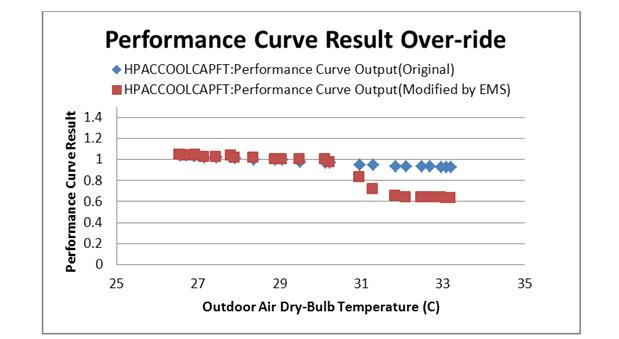
\includegraphics[width=0.9\textwidth, height=0.9\textheight, keepaspectratio=true]{media/image011.jpg}
\caption{Results of Performance Curve Override \protect \label{fig:results-of-performance-curve-override}}
\end{figure}
